% Main document for the thesis. Compile from this directory.
\documentclass[a4paper,11pt,titlepage,twoside,openany]{book}

\usepackage[T1]{fontenc}
\usepackage[utf8]{inputenc}
\usepackage[english]{babel}
\usepackage{newtxtext,newtxmath}
\usepackage{microtype}
\usepackage{setspace}
\usepackage{titlesec}
\usepackage[paperheight=29.7cm,paperwidth=21cm,outer=1.5cm,inner=2.5cm,top=2cm,bottom=2cm]{geometry}
\usepackage{graphicx}
\usepackage{amsmath}
\usepackage{booktabs}
\usepackage{tabularx}
\usepackage{array}
\usepackage{multirow}
\usepackage{float}
\usepackage{xcolor}
\usepackage{caption}
\usepackage{subcaption}
\usepackage{url}
\usepackage[hidelinks]{hyperref}
\usepackage[capitalise,noabbrev]{cleveref}

\graphicspath{{./figures/}}
\setlength{\parindent}{1.2em}
\setlength{\parskip}{0.25em}
\setcounter{tocdepth}{2}
\setcounter{secnumdepth}{3}
\singlespacing
\emergencystretch=2em

\newcommand{\thesistitle}{Evolving Neuron-Centric Hebbian Learning for Soft-Robot Control}
\newcommand{\thesissubtitle}{Performance, robustness, and task-dependent adaptation in EvoGym}
\newcommand{\thesisauthor}{Rowan Li Tangalin}
\newcommand{\degreeprogramme}{Computer, Communications and Electronic Engineering}
\newcommand{\supervisorname}{Giovanni Iacca}
\newcommand{\academicyear}{2026/2027}

\newcommand{\nchl}{NcHL}
\newcommand{\staticcontroller}{Static-ES}
\newcommand{\nchlcontroller}{NcHL-ES}
\newcommand{\code}[1]{\texttt{#1}}

% EvoGym's standard voxel colours: rigid, soft, horizontal actuator, vertical actuator.
\definecolor{evorigid}{RGB}{38,38,38}
\definecolor{evosoft}{RGB}{191,191,191}
\definecolor{evohact}{RGB}{242,142,43}
\definecolor{evovact}{RGB}{56,119,222}
\newcommand{\voxelbox}[1]{%
  \begingroup
  \setlength{\fboxsep}{0pt}%
  \setlength{\fboxrule}{0.3pt}%
  \fcolorbox{black!55}{#1}{\rule{0pt}{4.3mm}\rule{4.3mm}{0pt}}%
  \endgroup}
\newcommand{\emptyvoxel}{\makebox[4.9mm][c]{\rule{0pt}{4.9mm}}}
\newcommand{\rigidvoxel}{\voxelbox{evorigid}}
\newcommand{\softvoxel}{\voxelbox{evosoft}}
\newcommand{\hactvoxel}{\voxelbox{evohact}}
\newcommand{\vactvoxel}{\voxelbox{evovact}}
\newcommand{\voxellegend}{%
  \small
  \rigidvoxel\ Rigid\quad
  \softvoxel\ Soft\quad
  \hactvoxel\ Horizontal actuator\quad
  \vactvoxel\ Vertical actuator}
\begin{document}
\pagenumbering{gobble}
\pagestyle{plain}

\thispagestyle{empty}


\begin{center}
  
\includegraphics[width=0.6\textwidth]{marchio_unitrento_colore_it_202002-eps-converted-to.pdf}

  \vspace{2 cm} 
    {\Large Department of Information Engineering and Computer Science\\}
    \vspace{0.65cm}
    {\large Bachelor's Degree in \degreeprogramme\\}

    \vspace{2 cm} 
    {\large Final Dissertation\\}
    \vspace{1cm}
    {\Huge\textsc \thesistitle}

    \vspace{2cm}
  \begin{tabular*}{\textwidth}{ c @{\extracolsep{\fill}} c }
      \textbf{Supervisor} & \textbf{Student} \\
      \supervisorname & \thesisauthor
    \end{tabular*}

    \vspace{2cm}
    {\large Academic year \academicyear\par}

\end{center}

\clearpage
\chapter*{Acknowledgements}

\emph{To be completed.}

\clearpage
\pagestyle{plain}
\mainmatter
\tableofcontents
\clearpage

\begingroup
  \renewcommand{\cleardoublepage}{}
  \renewcommand{\clearpage}{}
  \titleformat{\chapter}
    {\normalfont\Huge\bfseries}{\thechapter}{1em}{}
  \titlespacing*{\chapter}{0pt}{0.59in}{0.02in}
  \titlespacing*{\section}{0pt}{0.20in}{0.02in}
  \titlespacing*{\subsection}{0pt}{0.10in}{0.02in}

  \chapter*{Use of Artificial Intelligence Tools}
\addcontentsline{toc}{chapter}{Use of Artificial Intelligence Tools}

OpenAI Codex was used to support language revision of the thesis, figure preparation, and plotting. 
\par
  \chapter*{Abstract}
\addcontentsline{toc}{chapter}{Abstract}

Soft robotics refers to the study of robotic systems that exploit deformable bodies in order to interact with complex environments. The same characteristics which enable these capabilities also make the systems more difficult to control. Additionally, certain applications of soft robotics, such as search-and-rescue in unstructured terrain, may benefit from the ability to adapt and learn during the lifetime of the robot in order to face unforeseen changes or simply optimize their behavior.

Biological systems achieve adaptability in part through synaptic plasticity, where the connections between neurons change according to their activity. Hebbian Learning provides a simple model of this principle by modifying neural-network weights online according to the activation of connected neurons. 

Conventional Hebbian formulations associate plasticity parameters with individual synapses, causing the number of parameters to grow with the number of connections. Neuron-centric Hebbian Learning (NcHL) addresses this scaling problem by associating the parameters governing plasticity with the neurons instead, substantially reducing the dimensionality of the learning rule while preserving activity-dependent adaptation.

This project investigates whether NcHL can provide competitive and adaptive control for soft robots. In particular, we compare NcHL-based controllers with static neural controllers across different tasks and morphologies, examine the robustness of evolved NcHL rules to unseen neural-network initializations, and investigate whether NcHL produces meaningful learning within an individual lifetime.

The second, larger experiment extends the controller comparison to twelve tasks and three controlled morphologies. Tasks are grouped in advance by dominant control demand---continuous-support locomotion, terrain negotiation, object interaction, and whole-body dynamic control---so that the analysis can test whether the relative performance of \nchl{} follows an interpretable task-level pattern.
\par
  \chapter{Introduction}
\label{cha:introduction}

Soft robots exploit deformable bodies to interact with environments in ways that are difficult for rigid mechanisms. Their compliance can support safe contact and adaptation to irregular terrain, but it also couples sensing, control, and body dynamics tightly~\cite{rus2015softrobots}. An autonomous soft robot is therefore useful only while the relationship between its sensors, controller, morphology, and environment remains suitable for the task.

However, conventional optimization usually produces controller parameters that remain fixed after training. The controller may generate different actions for different observations, but the mechanism that maps observations to actions cannot itself adapt during deployment. This is a restrictive assumption when the robot encounters changes that were absent from training, and it is especially relevant for soft bodies whose physical response is difficult to model precisely. Evolved plastic neural controllers address this problem by separating two processes: evolution searches across generations for a learning rule, and that rule modifies network weights during the lifetime of an individual~\cite{soltoggio2018borntolearn}.

\section{Research Questions and Contributions}

This thesis investigates Neuron-centric Hebbian Learning (\nchl), which reduces the number of evolved plasticity parameters by associating them with neurons rather than individual synapses~\cite{ferigo2024nchl}. It compares an evolved \nchl{} controller with a static neural controller while holding the morphology, observations, action mapping, network topology, evolutionary optimizer, and task horizon fixed within each experimental condition. The investigation is organized around four research questions.

\paragraph{RQ1 --- Evolutionary training dynamics.}
How does the best-so-far fitness of \nchlcontroller{} develop during evolution relative to Static-ES across the original task--morphology conditions?

\paragraph{RQ2 --- Robustness to initialization.}
Does an evolved \nchl{} rule remain effective when the concrete neural-network weights are initialized with random seeds not encountered during evolution?

\paragraph{RQ3 --- Within-lifetime learning.}
Do the weight updates produced by \nchl{} create behaviourally useful weights, as opposed to weight change without a corresponding performance benefit?

\paragraph{RQ4 --- Task and morphology dependence.}
Which task characteristics are associated with good \nchl{} performance, and are those patterns independent of morphology?


The thesis makes three principal contributions:
\begin{enumerate}
  \item A controlled comparison of \nchlcontroller{} and Static-ES on the original EvoGym task and morphology suite, including evolutionary training dynamics and qualitative inspection of the evolved behaviour;
  \item Two mechanistic evaluations of the learned plasticity rules, testing sensitivity to unseen initial weights and whether weights acquired during a lifetime remain useful when frozen and replayed;
  \item An extension to twelve tasks and three controlled morphologies, combining task-group analysis, task--morphology comparisons, and controller footage to investigate whether \nchl{} performance follows task characteristics or body geometry.
\end{enumerate}

The study validates these contributions with ten independent evolutionary runs per condition, generation-level fitness curves, evaluations across unseen initializations, freeze-and-replay interventions, standardized comparisons across task-specific reward scales, and qualitative footage analysis. The results show that \nchl{} can produce meaningful locomotion and object-interaction behaviour, and that its online updates often improve on random initial weights. They also show sensitivity to initialization, no consistent task-class advantage, and a substantially clear dependence on morphology.

\section{Thesis Outline}

\Cref{cha:background} introduces EvoGym, Hebbian learning, \nchl{}, and the evolutionary optimizer used in the experiments. \Cref{cha:original-study} presents the original study and answers RQ1--RQ3 through its methodology and results. \Cref{cha:extended} extends the comparison across tasks and controlled morphologies and answers RQ4. \Cref{cha:discussion} summarizes the conclusions, limitations, and directions for future work.
\par
  \chapter{Background}
\label{cha:background}

\section{EvoGym}

Evolution Gym, usually shortened to EvoGym, is a benchmark for the joint optimization of the design and control of two-dimensional soft robots~\cite{bhatia2021evolution}. It provides a common representation for robot bodies and a collection of environments in which those bodies can be controlled. Its simulator models voxel-based objects using an underlying mass--spring system, advances their physical state over discrete timesteps, and exposes the resulting control problem through a Gym-compatible interface.

An EvoGym interaction follows the usual agent--environment loop. At timestep $t$, the environment provides an observation $\mathbf{o}_t$. The controller maps it to an action $\mathbf{u}_t$, which specifies a deformation scale for each of the robot's actuators. After simulating the action, the environment returns a new observation, a scalar reward $r_t$, and an indication of whether the episode has ended. The return of one episode is
\begin{equation}
  F = \sum_{t=0}^{T-1} r_t,
  \label{eq:return}
\end{equation}
where $T$ is the episode horizon or the timestep at which the environment terminates. This return is used as fitness by the evolutionary optimizer~\cite{bhatia2021evolution}.

EvoGym is useful for this project because it separates three objects that need to remain conceptually distinct: morphology, task, and controller. Holding two of these objects fixed facilitates the study of the third.

\subsection{Morphologies}

An EvoGym morphology is a rectangular matrix of integer material codes. Each non-empty matrix cell represents one square voxel. Adjacent occupied cells are connected in the physical simulation, so the matrix specifies both the material distribution and the geometry of the robot. A valid robot body must form one connected structure and must contain at least one actuator~\cite{bhatia2021evolution}.

Table~\ref{tab:voxel-types} lists the material codes used by the morphologies in this thesis. Rigid voxels resist deformation and provide structural support. Soft voxels deform passively in response to forces. Horizontal and vertical actuators actively expand or contract along their named axis~\cite{bhatia2021evolution}.

\begin{table}[htbp]
  \centering
  \caption{EvoGym voxel codes used to describe robot morphologies.}
  \label{tab:voxel-types}
  \begin{tabularx}{0.9\textwidth}{@{}clX@{}}
    \toprule
    Code & Type & Role in a morphology \\
    \midrule
    0 & Empty & No robot material is placed in the cell. \\
    1 & Rigid & Provides an occupied, non-deformable structural element. \\
    2 & Soft & Deforms passively under internal and external forces. \\
    3 & Horizontal actuator & Changes its preferred width in response to a control signal. \\
    4 & Vertical actuator & Changes its preferred height in response to a control signal. \\
    \bottomrule
  \end{tabularx}
\end{table}

The number of actuators determines the size of the controller's output, while the number and arrangement of voxels affect the observation and the physical consequences of each action.

\subsection{Tasks}

In EvoGym, a task defines the terrain and other simulated objects, the initial placement of the robot, the observations available to the controller, the admissible actuator commands, the reward calculated after each transition, and the conditions that terminate an episode.

Observations contain task-specific information about the robot and the surrounding world. Typical robot information includes velocities and the positions of voxel corner masses relative to the robot's centre of mass. Environments that contain a movable object or a target can add relative positions, object velocities, or other quantities required to make progress observable. The observation is presented to the controller as a numerical vector and the controller is not given a symbolic description of the task.

The action vector contains one command for every actuator voxel in the morphology. A command changes the actuator's target length, causing expansion or contraction. Useful motion must emerge from the timing of these local deformations, the passive response of the body, and contact with the environment. Rigid and passive soft voxels do not receive commands.

Reward gives numerical feedback about progress. Its definition is part of the task: it may value displacement, object motion, height, reaching a target, or a combination of several terms. Consequently, return is meaningful within a task but is not a universal unit of performance. A return of a particular magnitude in one EvoGym environment cannot be interpreted as better than the same number in another environment without an explicit normalization~\cite{bhatia2021evolution}.

\section{Hebbian Learning}

Hebbian learning is a concept built around manipulating synaptic weight based on the activation of the two neurons connected by that synapse. Unlike supervised backpropagation, a Hebbian update does not require a target output or the gradient of a global loss. The central idea is to use a learning rule to produce useful updates to the weights of the network based on its own current state and observations~\cite{ferigo2024nchl,ferigo2023voxelhebbian}.

\subsection{ABCD Hebbian Learning Rules}

A generalized ABCD rule represents four basic influences on a connection from presynaptic neuron $i$ to postsynaptic neuron $j$~\cite{ferigo2024nchl,ferigo2023voxelhebbian}:
\begin{equation}
  \Delta w_{ij} = \eta\left(
    A_{ij}a_i + B_{ij}a_j + C_{ij}a_i a_j + D_{ij}
  \right),
  \label{eq:abcd}
\end{equation}
where $a_i$ and $a_j$ are the current neuron activations and $\eta$ is a learning-rate scale. The $A$ and $B$ terms depend on the presynaptic and postsynaptic activity, respectively. The $C$ term can reinforce or suppress a connection according to joint activity, while $D$ allows activation-independent changes.

\subsection{Neuron-centric Hebbian Learning}

Neuron-centric Hebbian Learning moves the evolved parameters from synapses to neurons~\cite{ferigo2024nchl}. In the published formulation, each neuron $k$ stores one tuple
\begin{equation}
  \boldsymbol{\theta}_k=(A_k,B_k,C_k,D_k,\eta_k).
\end{equation}
The update for a connection is assembled from the tuples belonging to its presynaptic and postsynaptic endpoints. The rule uses the mean of their learning rates:
\begin{equation}
  \Delta w_{ij}=\frac{\eta_i+\eta_j}{2}\left(
    A_i a_i + B_j a_j + C_iC_j a_i a_j + D_iD_j
  \right).
  \label{eq:nchl-published}
\end{equation}

\section{Evolution}

Evolutionary computation searches over a population of candidate solutions using fitness evaluation, selection, and variation, without requiring gradient information~\cite{eiben2015evolutionary}. This is useful in EvoGym because fitness depends on a simulated trajectory containing contacts, deformation, and many successive controller decisions. It is also useful for plastic controllers: evolution can optimize the coefficients of a learning rule using only the fitness of the individual.

In the terminology used here, a \emph{genome} is the numerical vector inherited and modified by the optimizer, an \emph{individual} is one candidate genome, and a \emph{population} is the set of candidates evaluated in a generation. The meaning of a gene depends on the controller representation. A static genome stores connection weights. An \nchl{} genome stores neuron-level learning-rule coefficients. In both cases, EvoGym episode return supplies the fitness used to rank candidates.

\subsection{Genetic Algorithms}

A Genetic Algorithm (GA) is a population-based evolutionary algorithm built around repeated evaluation, selection, and variation. An initial population is generated, every individual is assigned a fitness, and better-performing individuals are given a greater role in producing the next generation. Variation operators such as mutation and crossover create new genomes from the selected parents. The cycle continues until an evaluation budget or another stopping condition is reached.

Selection makes the search exploit information already discovered, while variation explores nearby or recombined solutions. Mutation changes genes stochastically; crossover combines material from multiple parents. Elitism may copy one or more strong individuals unchanged so that an already discovered solution is not lost through random variation.

These components describe a large family of mathematical algorithms which can work in discrete or continuous domains. Specific evolutionary optimizers choose different representations, selection rules, and variation distributions~\cite{eiben2015evolutionary}.

\subsection{ES1}

ES1 is the chosen strategy; it uses the arithmetic mean of the best $\mu$ genomes. If $\mathbf{g}_1,\ldots,\mathbf{g}_\mu$ are the selected parents, their centre is
\begin{equation}
  \bar{\mathbf{g}}=\frac{1}{\mu}\sum_{i=1}^{\mu}\mathbf{g}_i.
\end{equation}
Each new candidate is sampled by adding isotropic Gaussian noise,
\begin{equation}
  \mathbf{g}'=\bar{\mathbf{g}}+\sigma\boldsymbol{\epsilon},
  \qquad \boldsymbol{\epsilon}\sim\mathcal{N}(\mathbf{0},I),
  \label{eq:es1}
\end{equation}
where $\sigma$ controls the mutation scale. The best genome encountered so far is retained unchanged through elitism. Unlike a GA with crossover, ES1 does not preserve and recombine discrete parent genomes. It summarizes the selected set by its mean and explores a neighbourhood around that point.
\par
  \chapter{Original Study: Methodology and Results}
\label{cha:original-study}

This chapter presents the completed original study as three linked experiments. \Cref{sec:shared-framework} defines the implementation, controllers, tasks, and protocol that all three experiments share. \Cref{sec:rq1} compares held-out performance, \Cref{sec:rq2} tests robustness to unseen initial weights, and \Cref{sec:rq3} examines whether lifetime updates create reusable weights.
\section{Shared Experimental Framework}
\label{sec:shared-framework}

\subsection{Implementation and Reproducibility}

Python implements the experiments, Gymnasium exposes the EvoGym environments, and PyTorch networks control the robots. A YAML configuration records the task, morphology, controller, network, evolutionary budget, evaluation protocol, runtime settings, and training seed. Before training, the implementation resolves symbolic network dimensions against the instantiated environment.

The implementation uses separate run seeds. Optimizer sampling, environment resets, and \nchl{} weight initialization therefore do not share one global generator. Before each reset, the implementation also reseeds the global Python generator for EvoGym tasks that use it internally. BidirectionalWalker, for example, selects its target direction during reset.

Each completed run stores a resolved configuration, generation-level metrics and the best genome.

\subsection{Controller Implementations}

Both conditions use the same bias-free feed-forward topology. The instantiated task and morphology determine the input width. The network contains one hidden layer with the same width as the observation vector and one output for each actuator voxel. Every layer applies a hyperbolic tangent activation:
\begin{equation}
  \mathbf{a}^{(\ell+1)}=\tanh\!\left(W^{(\ell)}\mathbf{a}^{(\ell)}\right).
  \label{eq:forward}
\end{equation}
The domain of the output is $[-1,1]$. A piecewise-linear transformation maps zero to the neutral actuator target $1.0$, negative values towards the lower action bound, and positive values towards the upper bound. This transformation preserves a meaningful neutral command when the bounds are asymmetric.

For raw network output $a_i\in[-1,1]$, lower bound $l_i$, and upper bound $u_i$, the physical actuator command is
\begin{equation}
  \widetilde{a}_i=
  \begin{cases}
    1+(1-l_i)a_i, & -1\leq a_i<0,\\
    1+(u_i-1)a_i, & 0\leq a_i\leq 1.
  \end{cases}
  \label{eq:action-mapping}
\end{equation}
Thus $a_i=-1$, $0$, and $1$ map exactly to $l_i$, $1.0$, and $u_i$, respectively.

The static condition evolves every matrix entry and loads the resulting values at the start of an episode. These weights remain fixed. The \nchl{} condition evolves per neuron parameters and samples concrete weights independently from a configured uniform interval at every episode reset. After each forward pass, the controller immediately applies the update with the pre- and postsynaptic activations cached during that pass.

The representations differ in genome length and evaluation budget, therefore the test is not a fixed compute comparison. \Cref{tab:original-settings} reports both shared and controller-specific settings.

\subsection{Tasks, Morphologies, and Evolution}

The original suite contains Walker-v0, Carrier-v0, Jumper-v0, and Thrower-v0. Every task uses the biped body; Thrower also uses a specialized arm. The two Thrower bodies differ in size and actuator count, so their comparison remains descriptive rather than controlled and is simply a study into the effect of morphology.

\begin{table}[htbp]
  \centering
  \caption{Original task--morphology conditions. The names follow the archived run configurations.}
  \label{tab:original-strata}
  \begin{tabularx}{\textwidth}{@{}llrX@{}}
    \toprule
    Task & Morphology & Horizon & Principal Behaviour \\
    \midrule
    Walker-v0 & biped & 500 & Forward locomotion on flat terrain \\
    Carrier-v0 & biped & 500 & Object transport during locomotion \\
    Jumper-v0 & biped & 500 & Vertical impulse generation \\
    Thrower-v0 & biped & 300 & Object acceleration and release \\
    Thrower-v0 & thrower\_arm & 300 & Throwing with specialized geometry \\
    \bottomrule
  \end{tabularx}
\end{table}

\begin{figure}[htbp]
  \centering
  \begin{subfigure}[t]{0.42\textwidth}
    \centering
    \setlength{\tabcolsep}{0pt}
    \begin{tabular}{cccc}
      \hactvoxel&\vactvoxel&\hactvoxel&\vactvoxel\\
      \hactvoxel&\rigidvoxel&\rigidvoxel&\vactvoxel\\
      \hactvoxel&\emptyvoxel&\emptyvoxel&\vactvoxel
    \end{tabular}
    \caption{Original-study biped.}
  \end{subfigure}
  \hfill
  \begin{subfigure}[t]{0.42\textwidth}
    \centering
    \setlength{\tabcolsep}{0pt}
    \begin{tabular}{cccccc}
      \emptyvoxel&\emptyvoxel&\rigidvoxel&\rigidvoxel&\hactvoxel&\hactvoxel\\
      \emptyvoxel&\rigidvoxel&\softvoxel&\hactvoxel&\vactvoxel&\hactvoxel\\
      \rigidvoxel&\vactvoxel&\hactvoxel&\softvoxel&\vactvoxel&\rigidvoxel\\
      \vactvoxel&\hactvoxel&\vactvoxel&\hactvoxel&\vactvoxel&\emptyvoxel\\
      \vactvoxel&\emptyvoxel&\vactvoxel&\emptyvoxel&\vactvoxel&\emptyvoxel\\
      \vactvoxel&\emptyvoxel&\vactvoxel&\emptyvoxel&\vactvoxel&\emptyvoxel
    \end{tabular}
    \caption{Specialized thrower arm.}
  \end{subfigure}

  \medskip
  \voxellegend
  \caption{Morphologies used in the original study.}
  \label{fig:original-bodies}
\end{figure}

Each combination of task, morphology, controller, and seed forms an independent optimization run. Both conditions use a population of 40 for 500 generations, select ten parents, apply Gaussian perturbation with $\sigma=0.35$, and retain the best genome observed so far. Static candidate fitness uses one episode. \nchl{} candidate fitness uses the mean of three episodes with distinct initialization and environment seed pairs in an attempt to generalize the rule across initializations.

\begin{table}[htbp]
  \centering
  \caption{Shared and controller-specific settings in the original study.}
  \label{tab:original-settings}
  \begin{tabularx}{0.94\textwidth}{@{}lX@{}}
    \toprule
    Item & Value \\
    \midrule
    Optimizer & ES1 with parent-mean Gaussian sampling and elitism \\
    Population and generations & 40 candidates and 500 generations \\
    Parent count and mutation scale & $\mu=10$ and $\sigma=0.35$ \\
    Initial evolutionary population & Uniform samples from $[-1,1]$ \\
    Candidate budget & One episode for Static-ES; three for \nchlcontroller \\
    Initial \nchl{} runtime weights & Independent uniform samples from $[-0.1,0.1]$ \\
    \nchl{} learning rate & $\eta=0.1$ \\
    Held-out evaluation & Ten episodes for each selected genome \\
    Training seeds & 0--9 \\
    \bottomrule
  \end{tabularx}
\end{table}

The evidence comprises 100 evolutionary runs, 1,000 held-out episodes, 300 weight traces, and 750 frozen-controller rollouts. The candidate evaluations add four million nested training episodes. All principal analyses use a trained run as the independent unit.

\section{RQ1: Evolutionary Training Dynamics}
\label{sec:rq1}

\subsection{Experimental Design}

This experiment uses the generation-level metrics from the ten independent evolutionary runs for each controller and task--morphology condition. At every generation, the analysis records the best fitness in the current population, the best fitness observed so far, and the population median. The curves summarize the across-run mean best-so-far fitness with a bootstrap interval and show the mean population median as a dashed line.

To determine whether the numerical fitness corresponds to recognizable task behaviour, an inspection of the footage of the best saved controller from each seed was performed. This visual assessment is qualitative: it helps distinguish genuine task completion from reward improvement that does not produce the intended behaviour.

\begin{figure}[htbp]
  \centering
  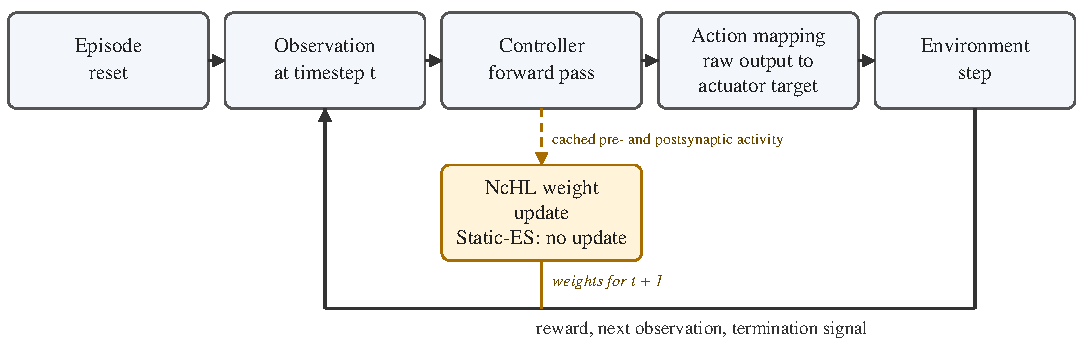
\includegraphics[width=\textwidth]{figures/training_loop.pdf}
  \caption{Within-episode control loop used to evaluate one candidate. The loop repeats until termination; accumulated reward becomes candidate fitness. The lower branch shows the additional online update performed only by \nchlcontroller.}
  \label{fig:training-loop}
\end{figure}

\subsection{Results}

The evolutionary curves show improvement for both representations. \nchlcontroller{} reaches a mean selected training fitness 4.2\% above Static-ES on Walker and 55.1\% above it on Jumper. Static-ES finishes higher on Carrier and both Thrower morphologies. \Cref{fig:evolutionary-trends} also shows substantial variation across independent runs, particularly for \nchlcontroller{}.

\begin{figure}[htbp]
  \centering
  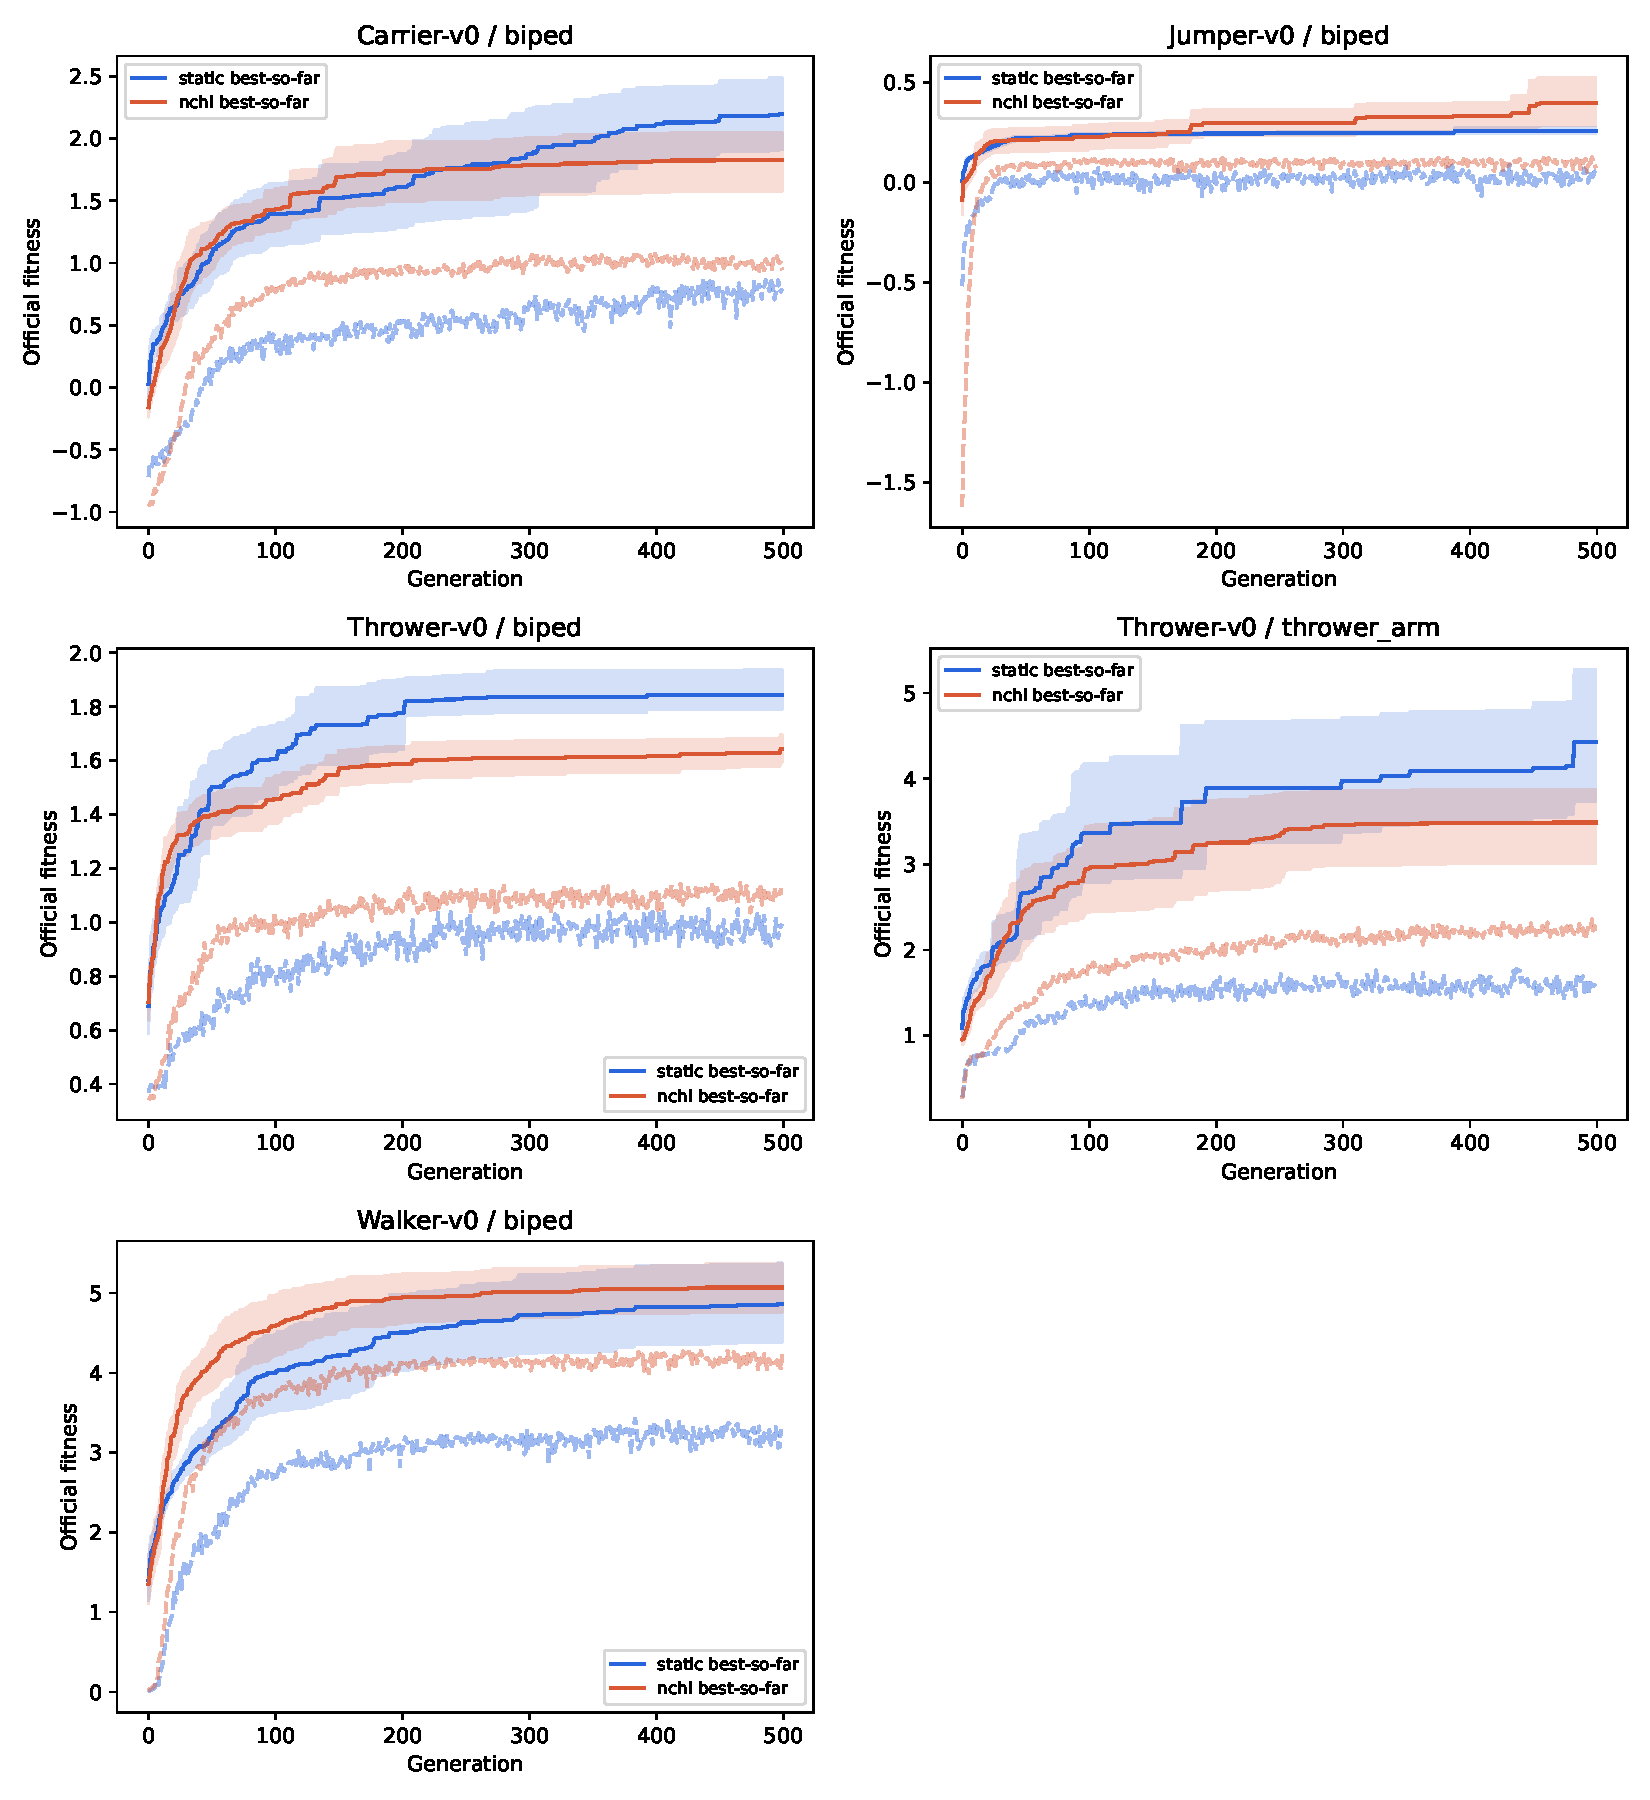
\includegraphics[width=0.98\textwidth]{figures/evolutionary_trends.pdf}
  \caption{Evolutionary training dynamics across ten runs per controller and condition. Solid lines show mean best-so-far fitness, shaded regions show bootstrap intervals, and dashed lines show the mean population median.}
  \label{fig:evolutionary-trends}
\end{figure}

The footage provides important context for these curves. On Walker, most seeds of both \nchlcontroller{} and Static-ES produce natural-looking locomotion. The biped and specialized-arm Thrower controllers can load the box and then release it with a recognizable throwing movement. These successful conditions show that \nchl{} can support both cyclical locomotion and non-cyclical, phase-structured behaviour.

Carrier and Jumper do not provide equally strong evidence. The Carrier controllers drop the box almost immediately, whereas the Jumper controllers consistently stretch upwards and then freeze; only the best examples produce a small jump. The tested morphologies and training setup therefore fail to solve these two tasks in behavioural terms. Their fitness curves still describe optimization under the task reward, but differences between \nchlcontroller{} and Static-ES in these conditions should not be treated as strong evidence about controller capability. In particular, the numerical \nchl{} advantage on Jumper does not correspond to a convincing solution of the task.

\paragraph{RQ1 Summary.} Both representations improve during evolution, but the fitness curves do not always indicate successful task behaviour. Walker and both Thrower morphologies produce meaningful solutions, demonstrating that \nchl{} can support both cyclical and phase-structured control. Carrier and Jumper remain behaviourally unsolved with the tested morphologies, so their relative fitness values provide weak evidence for comparing the controllers.

\clearpage
\section{RQ2: Robustness to Unseen Initial Weights}
\label{sec:rq2}

\subsection{Experimental Design}

An \nchl{} genome encodes a rule rather than one final weight matrix. This experiment applies every selected rule to initial weights generated from seeds outside its training stream. The ten held-out episodes for each run vary both the environment seed and controller seed. Because the original nominal environments behave deterministically after their declared reset, the sampled runtime weights dominate the additional within-run dispersion.

We compare the selected training fitness for each run---the maximum three-episode candidate estimate observed during evolution---with the mean over ten held-out initializations. The difference addresses practical generalization but can combine three mechanisms: specialization to fixed training pairs, optimism from selecting the maximum noisy estimate, and an inability to recover from arbitrary $W_0$. This design establishes the gap but cannot separate those causes.

\subsection{Results}

All 50 selected \nchl{} solutions achieve a lower mean across ten unseen initial weights than their selected three-initialization training estimate. \Cref{tab:rq2-generalization} reports the condition means. Retained performance divides the held-out mean by the selected training mean.

\begin{table}[htbp]
  \centering
  \small
  \caption{Generalization of selected \nchl{} rules to unseen runtime-weight initializations. Within-run SD summarizes ten nested episodes.}
  \label{tab:rq2-generalization}
  \begin{tabular}{@{}lrrrrrr@{}}
    \toprule
    Condition & Training & Held-out & Gap & Retained & Within-run SD & Negative Episodes \\
    \midrule
    Walker, biped & 5.069 & 4.395 & $-0.674$ & 86.7\% & 0.691 & 1/100 \\
    Carrier, biped & 1.825 & 1.191 & $-0.634$ & 65.3\% & 0.464 & 3/100 \\
    Jumper, biped & 0.399 & 0.024 & $-0.375$ & 6.0\% & 0.369 & 35/100 \\
    Thrower, biped & 1.643 & 1.215 & $-0.429$ & 73.9\% & 0.289 & 2/100 \\
    Thrower, arm & 3.488 & 2.233 & $-1.255$ & 64.0\% & 0.613 & 8/100 \\
    \bottomrule
  \end{tabular}
\end{table}

Jumper provides the strongest failure case. Its held-out mean retains only 6.0\% of the selected training mean, four of ten run means become negative, and 35 of 100 nested episodes produce negative return. Walker retains 86.7\%, whereas Carrier and the two Thrower conditions retain approximately 64--74\%. Static-ES reproduces its selected weights during evaluation and therefore has no corresponding variation from weight initialization.

Evolution evaluates three fixed initialization pairs per run and selects the best noisy candidate encountered across 500 generations. Lower held-out performance can therefore reflect specialization, selection optimism, or insufficient recovery from arbitrary starting weights. The data establish the practical result that new runtime weights remain consequential in every condition.

\paragraph{RQ2 Summary.} The results indicate that weight initialization influences the behaviour produced by the evolved learning rules. Nevertheless, the Walker and Thrower controllers retain meaningful task behaviour across initializations, suggesting that the rules capture useful structure rather than relying on a single favourable initialization. The poor performance on Carrier and Jumper is less informative about robustness because these tasks were not successfully learned under the nominal evaluation either.

\section{RQ3: Do Lifetime Updates Create Useful Weights?}
\label{sec:rq3}

\subsection{Freeze-and-Replay Design}

This experiment reuses the best \nchl{} genome from every original run and performs no further evolutionary search. Three independently seeded plastic source episodes generate concrete weight matrices at five normalized lifetime positions:
\begin{equation}
  W_0,\quad W_{25},\quad W_{50},\quad W_{75},\quad W_{\mathrm{final}}.
\end{equation}
The trace records $W_0$ before the first action. It records $W_{\mathrm{final}}$ after the update that follows the last source action, so this final matrix might never generate an action in the source trajectory.

The replay procedure loads each matrix into a static network and starts a fresh episode with the environment seed of the corresponding source trace. It disables plasticity throughout replay. This intervention tests whether an acquired matrix remains useful from the normal initial state; it does not continue from the physical state that produced the matrix.

For every snapshot, we first average the three traces within each evolutionary run and then summarize the runs. The principal quantities are the frozen-fitness change from $W_0$, the lifetime stage with the best frozen fitness, and the difference between the fully plastic source return and each frozen controller. Improvement over $W_0$ supports lifetime improvement.

\subsection{Results}

The experiment starts from a deliberately weak baseline. Before adaptation, random $W_0$ networks produce near-zero Walker fitness, negative Carrier and Jumper fitness, and low Thrower fitness. Later snapshots acquire useful fresh-start behaviour in several conditions, but the pattern is neither uniform nor monotonic (\Cref{tab:rq3-freeze}).

\begin{table}[htbp]
  \centering
  \scriptsize
  \caption{Fresh-start frozen fitness across lifetime snapshots. Values first average three traces within each run and then average ten run means. ``Improved'' counts runs for which $W_{\mathrm{final}}$ exceeds $W_0$.}
  \label{tab:rq3-freeze}
  \begin{tabular}{@{}lrrrrrrrr@{}}
    \toprule
    Condition & Plastic & $W_0$ & $W_{25}$ & $W_{50}$ & $W_{75}$ & $W_{final}$ & Final Change & Improved \\
    \midrule
    Walker, biped & 4.557 & 0.000 & 2.263 & 2.242 & 2.030 & 2.381 & $+2.381$ & 8/10 \\
    Carrier, biped & 1.276 & $-0.490$ & $-0.083$ & $-0.019$ & $-0.017$ & 0.004 & $+0.493$ & 7/10 \\
    Jumper, biped & 0.167 & $-0.168$ & $-2.133$ & $-2.912$ & $-2.705$ & $-2.093$ & $-1.925$ & 0/10 \\
    Thrower, biped & 1.248 & 0.338 & 0.338 & 0.346 & 0.482 & 0.498 & $+0.160$ & 8/10 \\
    Thrower, arm & 2.252 & 0.243 & 1.087 & 1.037 & 1.172 & 1.369 & $+1.125$ & 9/10 \\
    \bottomrule
  \end{tabular}
\end{table}

\begin{figure}[htbp]
  \centering
  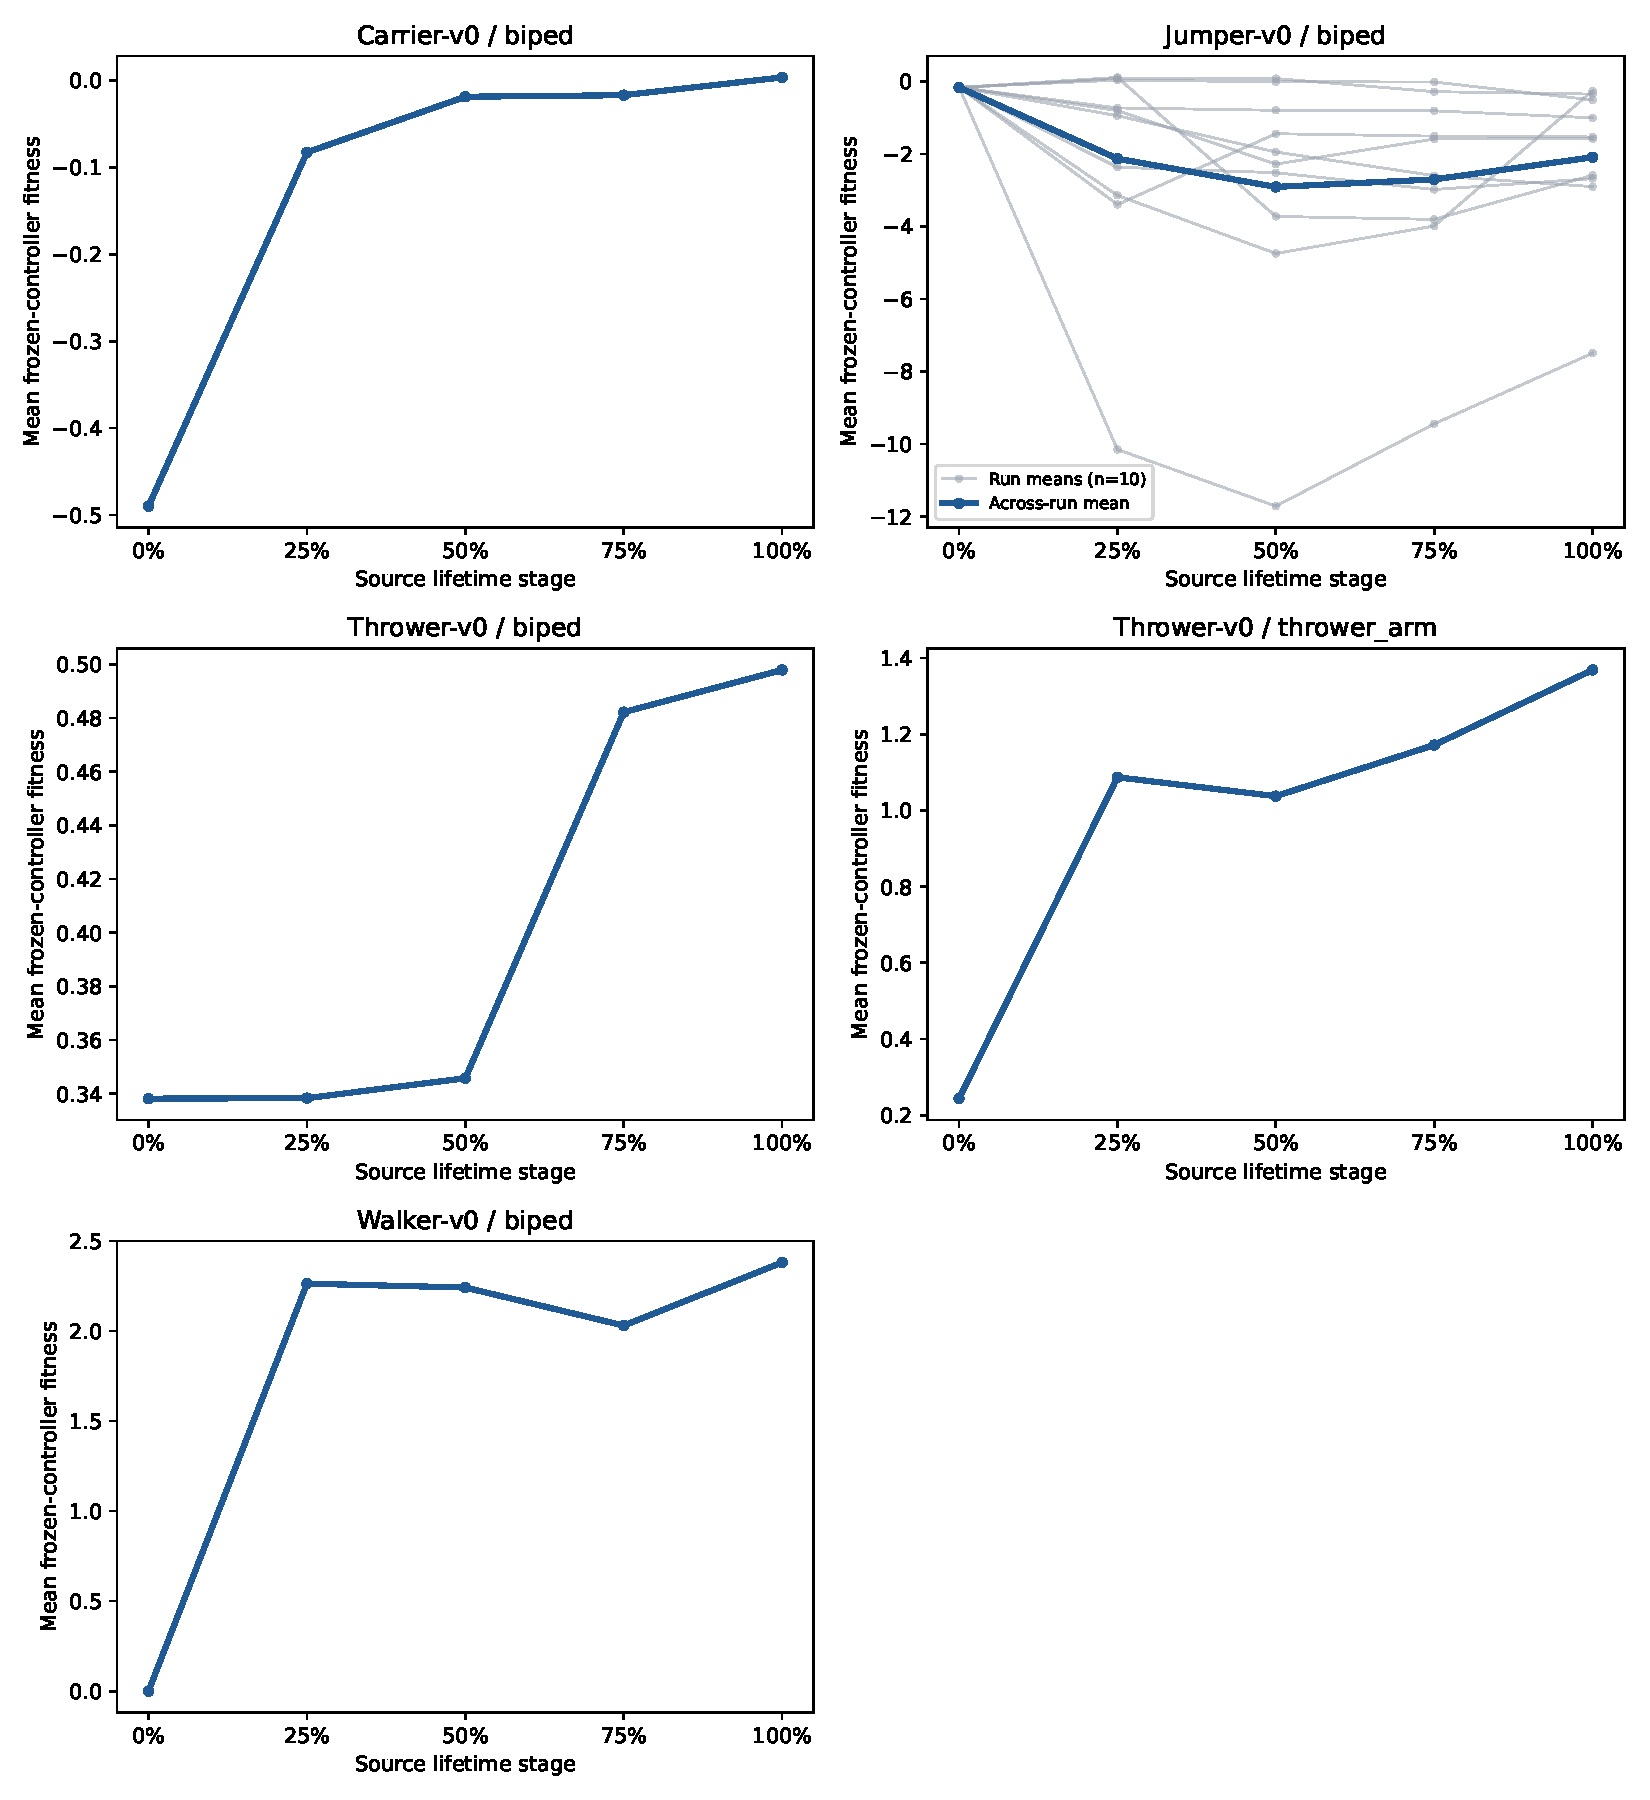
\includegraphics[width=0.98\textwidth]{figures/freeze_fitness_over_lifetime.pdf}
  \caption{Across-run mean fitness of frozen weight snapshots evaluated from a fresh task start. The Jumper panel retains the ten run means in grey to illustrate the large between-seed variation; the blue line gives the across-run mean in every panel.}
  \label{fig:freeze-fitness}
\end{figure}

Plastic control outperforms the matched $W_0$ frozen ablation in 49 of 50 runs. It also exceeds $W_{\mathrm{final}}$ in 47 runs and the post-hoc best frozen snapshot in 46. 

Only five of the 50 frozen trajectories improve monotonically across all five snapshots. The learning rule therefore does not simply approach one final static optimum. A late matrix can perform poorly from the initial physical state while remaining useful during the phase that produced it.

\paragraph{RQ3 Summary.} Online updates contribute to performance, but they do not generally converge towards one progressively better fixed controller. The Walker result however is interesting: its highest frozen fitness occurs at \(W_{\mathrm{final}}\), suggesting that tasks with periodic optimal movement may show an upward fitness trend as the repeated control loop is progressively optimized.

\par
  \chapter[Extended Study: Task and Morphology Dependence]{Extended Study: Task and\\Morphology Dependence}
\label{cha:extended}

\section{Motivation and Research Question}
\label{sec:extended-motivation}

The original study establishes that \nchl{} can evolve useful behaviour, but its small task set cannot show whether performance follows a general task property. The extended study addresses the limitations by comparing \nchlcontroller{} and Static-ES on twelve tasks and three controlled bodies.

This experiment answers RQ4: \emph{which task characteristics are associated with good \nchl{} performance, and are those patterns independent of morphology?} The chapter first reports the predefined group comparison and then uses individual tasks to interpret the physical and temporal demands behind it.

\section{Experimental Design}
\label{sec:extended-design}

\subsection{Task Selection and Predefined Groups}

The twelve environments were assigned to four groups before their results were inspected (\Cref{tab:extended-task-groups}). The groups describe a dominant control demand.

\begin{table}[htbp]
  \centering
  \small
  \caption{Predefined task groups in the extended experiment.}
  \label{tab:extended-task-groups}
  \begin{tabularx}{\textwidth}{@{}>{\raggedright\arraybackslash}p{0.22\textwidth}>{\raggedright\arraybackslash}p{0.35\textwidth}>{\raggedright\arraybackslash}X@{}}
    \toprule
    Group & Tasks & Dominant characteristic \\
    \midrule
    Continuous-support locomotion & Walker; BridgeWalker; BidirectionalWalker & Repeated locomotion on rigid or deformable support, including changing goals \\
    Terrain negotiation & DownStepper; ObstacleTraverser; CaveCrawler & Contact adaptation, terrain sensing, step transitions, and clearance control \\
    Object interaction & Pusher; Carrier; Thrower & Control while mechanically coupled to an external object \\
    Whole-body dynamic control & Flipper; Jumper; Balancer & Rotation, impulse generation, or postural regulation without sustained transport \\
    \bottomrule
  \end{tabularx}
\end{table}

\subsection{Control Demands of the Individual Tasks}

The group labels conceal differences that may matter to an activity-dependent controller. Based on the objectives and mechanics of the EvoGym environments, \Cref{tab:extended-task-demands} gives the author's classification of the principal temporal and physical demand of every task~\cite{bhatia2021evolution}. In particular, a repetitive task can retain one objective, as in Walker, or require repeated goal changes, as in BidirectionalWalker. Likewise, object interaction can require sustained contact or one precisely timed release.

\begin{table}[htbp]
  \centering
  \scriptsize
  \caption{Task characteristics used to interpret the controller comparison.}
  \label{tab:extended-task-demands}
  \begin{tabularx}{\textwidth}{@{}l>{\raggedright\arraybackslash}p{0.27\textwidth}>{\raggedright\arraybackslash}X@{}}
    \toprule
    Task & Temporal structure & Principal physical or control demand \\
    \midrule
    Walker & Repeated, fixed direction & Locomotion on rigid continuous support \\
    BridgeWalker & Repeated, fixed direction & Locomotion coupled to deformable support \\
    BidirectionalWalker & Sequential goals & Direction changes and context-dependent action \\
    DownStepper & Repeated with transitions & Descending contacts while remaining upright \\
    ObstacleTraverser & State-dependent & Terrain sensing, clearance, and balance \\
    CaveCrawler & Repeated under constraint & Simultaneous floor and ceiling clearance \\
    Pusher & Sustained progression & Persistent contact with a movable object \\
    Carrier & Sustained progression & Transport while retaining the load \\
    Thrower & Phase structured & Load, accelerate, and release \\
    Flipper & Repeated, one direction & Continued whole-body rotation \\
    Jumper & Ballistic & Compression, launch, and height retention \\
    Balancer & Stabilizing & Approach and maintain a target state \\
    \bottomrule
  \end{tabularx}
\end{table}

\subsection{Controlled Morphologies}

Every task is evaluated with a generalist biped, compact crawler, and hollow frame. Each body contains 24 occupied voxels: 12 rigid, two soft, five horizontal actuators, and five vertical actuators. The action dimension is therefore ten in every condition. Geometry and mass distribution change, while occupied volume, material counts, and actuator budget remain fixed.

\begin{figure}[htbp]
  \centering
  \begin{subfigure}[t]{0.31\textwidth}
    \centering
    \setlength{\tabcolsep}{0pt}
    \begin{tabular}{cccccc}
      \emptyvoxel&\rigidvoxel&\rigidvoxel&\rigidvoxel&\rigidvoxel&\emptyvoxel\\
      \hactvoxel&\vactvoxel&\rigidvoxel&\rigidvoxel&\hactvoxel&\vactvoxel\\
      \rigidvoxel&\hactvoxel&\softvoxel&\softvoxel&\vactvoxel&\rigidvoxel\\
      \vactvoxel&\hactvoxel&\emptyvoxel&\emptyvoxel&\vactvoxel&\hactvoxel\\
      \rigidvoxel&\rigidvoxel&\emptyvoxel&\emptyvoxel&\rigidvoxel&\rigidvoxel
    \end{tabular}
    \caption{Generalist biped.}
  \end{subfigure}
  \hfill
  \begin{subfigure}[t]{0.31\textwidth}
    \centering
    \setlength{\tabcolsep}{0pt}
    \begin{tabular}{cccccc}
      \rigidvoxel&\rigidvoxel&\rigidvoxel&\rigidvoxel&\rigidvoxel&\rigidvoxel\\
      \hactvoxel&\vactvoxel&\softvoxel&\softvoxel&\hactvoxel&\vactvoxel\\
      \rigidvoxel&\hactvoxel&\rigidvoxel&\rigidvoxel&\vactvoxel&\rigidvoxel\\
      \vactvoxel&\hactvoxel&\rigidvoxel&\rigidvoxel&\vactvoxel&\hactvoxel
    \end{tabular}
    \caption{Compact crawler.}
  \end{subfigure}
  \hfill
  \begin{subfigure}[t]{0.31\textwidth}
    \centering
    \setlength{\tabcolsep}{0pt}
    \begin{tabular}{cccccc}
      \emptyvoxel&\rigidvoxel&\rigidvoxel&\rigidvoxel&\rigidvoxel&\emptyvoxel\\
      \hactvoxel&\vactvoxel&\rigidvoxel&\rigidvoxel&\hactvoxel&\vactvoxel\\
      \rigidvoxel&\hactvoxel&\emptyvoxel&\emptyvoxel&\vactvoxel&\rigidvoxel\\
      \vactvoxel&\hactvoxel&\emptyvoxel&\emptyvoxel&\vactvoxel&\hactvoxel\\
      \rigidvoxel&\rigidvoxel&\softvoxel&\softvoxel&\rigidvoxel&\rigidvoxel
    \end{tabular}
    \caption{Hollow frame.}
  \end{subfigure}

  \medskip
  \voxellegend
  \caption{Controlled morphologies.}
  \label{fig:extended-bodies}
\end{figure}

The biped separates support into leg-like columns, the crawler forms a low and nearly rectangular contact structure, and the frame redistributes the same material around a central opening. 

\subsection{Experimental Scale and Completeness}

The design contains $12\times3\times2\times10=720$ independent optimization runs. Every run completed 500 generations with a population of 40 and mutation scale $0.35$. Static candidates use one episode, while \nchl{} candidates again average three runtime-weight initializations.

\section{Analysis Strategy}
\label{sec:extended-analysis}

The task-level curves first average the three morphology scores within each seed and then summarize the ten independent seeds. Their outcome is best-so-far fitness during evolution. Final comparisons use the selected best-so-far score at generation 500. Footage of the evolved controllers supplies a separate behavioural check: a higher task reward is not treated as evidence of controller capability when the robot is not able to perform the intended task recognizably. Numerical results from such conditions remain reported, but receive little weight.

Raw return is meaningful within a task but cannot be pooled across tasks. For task $t$, morphology $m$, and seed $s$, the controller difference is therefore standardized by the sample standard deviation of the 20 final scores in that task--morphology stratum:
\begin{equation}
  z_{tms}=
  \frac{F^{\nchl}_{tms}-F^{\mathrm{static}}_{tms}}{s_{tm}}.
  \label{eq:extended-standardized-effect}
\end{equation}
Positive values favour \nchlcontroller{} and negative values favour Static-ES. Group effects average the nine standardized values contributed by three tasks and three morphologies within each seed. Means are accompanied by non-parametric bootstrap intervals over the ten seed-level values. Raw within-task differences are retained where standardization could obscure practical magnitude.

\section{Results Across Tasks and Morphologies}
\label{sec:extended-results}

\subsection{Training Dynamics and Task-Group Results}

Both controller representations improve numerically on every task, but they do not reach the same training ceiling (\Cref{fig:extended-training-curves}). Walker, BridgeWalker, Pusher, Jumper, and CaveCrawler show rapid early gains followed by a plateau. Static-ES continues to separate on BidirectionalWalker, DownStepper, ObstacleTraverser, Carrier, Thrower, and Balancer. 

\begin{figure}[htbp]
  \centering
  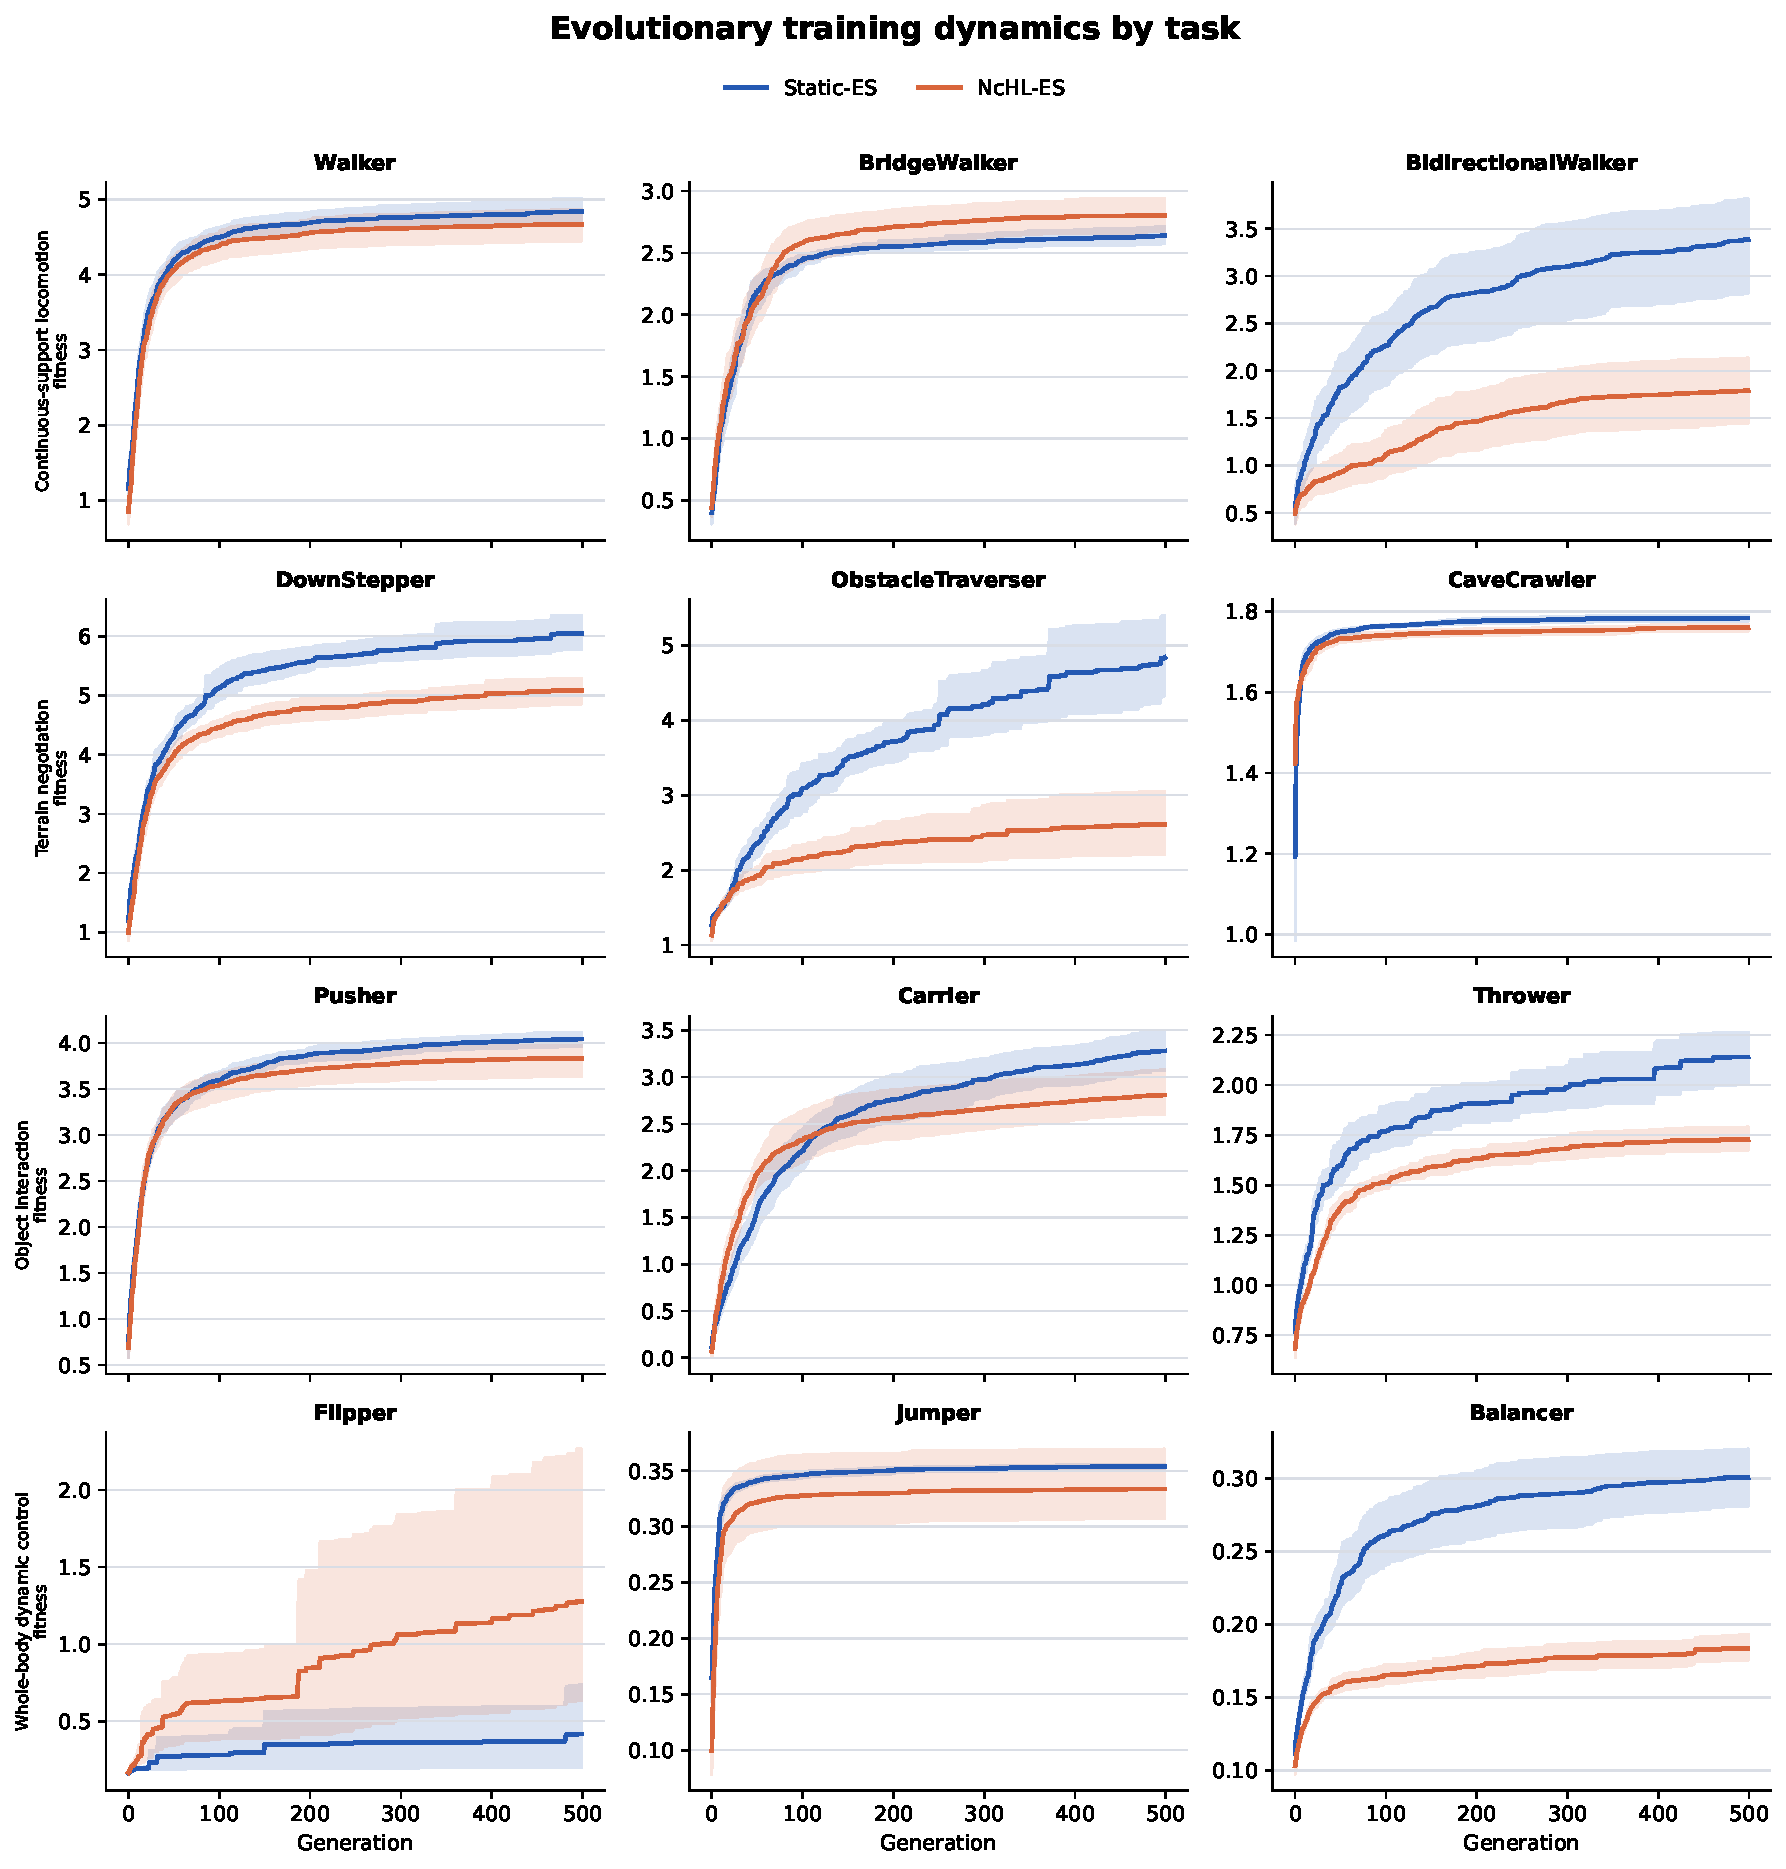
\includegraphics[width=0.98\textwidth]{figures/training_curves_by_task.pdf}
  \caption{Best-so-far evolutionary fitness for the twelve extended tasks. Each task curve first averages the three morphologies within a seed and then summarizes ten seeds; shaded bands are 95\% bootstrap intervals. Panels retain their task-specific reward scales.}
  \label{fig:extended-training-curves}
\end{figure}

None of the four predefined groups produce an aggregate \nchl{} advantage (\Cref{tab:extended-group-effects}). Terrain negotiation is most negative. Whole-body dynamic control is least negative numerically because the Flipper score partly offsets Jumper and Balancer. The footage prevents this offset from being interpreted as a positive behavioural result: none of the three whole-body tasks is learned recognizably.

\begin{table}[htbp]
  \centering
  \small
  \caption{Mean standardized final training effect by predefined task group. Positive values favour \nchlcontroller.}
  \label{tab:extended-group-effects}
  \begin{tabular}{@{}lrrr@{}}
    \toprule
    Group & Mean effect & 95\% interval & Positive seed effects \\
    \midrule
    Continuous-support locomotion & $-0.58$ & $[-0.70,-0.47]$ & 0/10 \\
    Terrain negotiation & $-1.15$ & $[-1.33,-0.91]$ & 0/10 \\
    Object interaction & $-0.67$ & $[-0.89,-0.40]$ & 1/10 \\
    Whole-body dynamic control & $-0.44$ & $[-0.77,-0.07]$ & 1/10 \\
    \bottomrule
  \end{tabular}
\end{table}

\Cref{tab:extended-footage} summarizes the behavioural evidence used to qualify these scores. 

\begin{table}[htbp]
  \centering
  \small
  \caption{Qualitative assessment of evolved-controller footage.}
  \label{tab:extended-footage}
  \begin{tabularx}{\textwidth}{@{}l>{\raggedright\arraybackslash}X>{\raggedright\arraybackslash}p{0.27\textwidth}@{}}
    \toprule
    Group & Observed behaviour & Interpretive weight \\
    \midrule
    Continuous-support locomotion & Controllers produce recognizable goal-directed locomotion & Informative \\
    Terrain negotiation & DownStepper is adequate; Static-ES performs acceptably on ObstacleTraverser while \nchl{} does not; CaveCrawler is not learned & Task-specific; CaveCrawler carries little weight \\
    Object interaction & Recognizable object-directed behaviour emerges & Informative \\
    Whole-body dynamic control & Flipper, Jumper, and Balancer are not learned recognizably & Low; fitness differences do not establish task competence \\
    \bottomrule
  \end{tabularx}
\end{table}

\subsection{Task-by-Morphology Results}

The aggregate group results conceal a strong interaction with body geometry (\Cref{fig:extended-endpoint-heatmap}). Only eight of the 36 numerical cells favour \nchl{}, and five of those use the compact crawler. Flipper is the only task with a positive score effect for every body, but its footage shows no successful solution. Conversely, BidirectionalWalker, DownStepper, ObstacleTraverser, CaveCrawler, Thrower, and Balancer are negative for all three morphologies.

\begin{figure}[htbp]
  \centering
  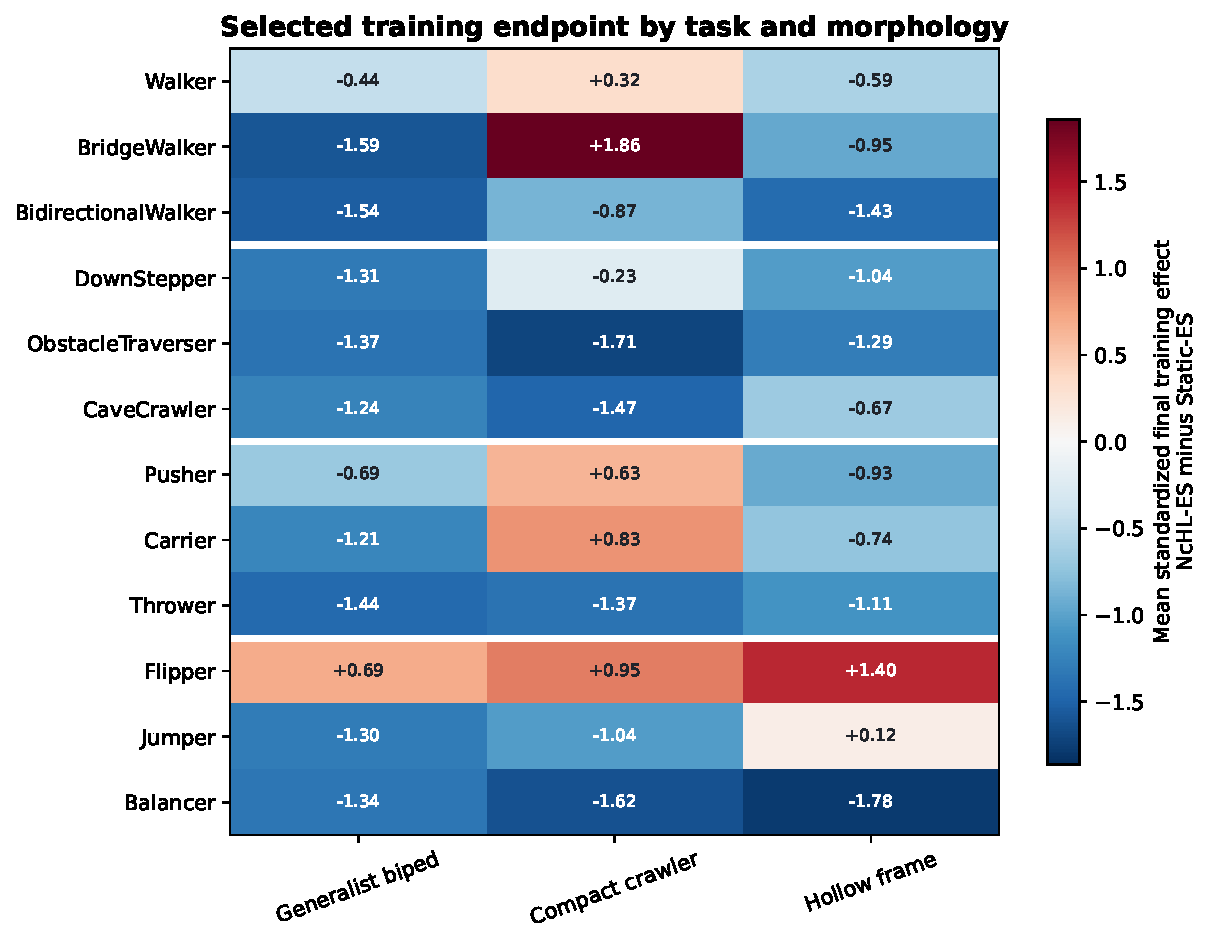
\includegraphics[width=0.86\textwidth]{figures/training_endpoint_heatmap.pdf}
  \caption{Mean standardized final training effect for every task--morphology condition. Positive values favour \nchlcontroller; negative values favour Static-ES. Horizontal separators indicate the four predefined task groups.}
  \label{fig:extended-endpoint-heatmap}
\end{figure}

\Cref{tab:extended-task-effects} summarizes the task averages and the morphology pattern behind them. BridgeWalker illustrates why both levels are required. Its raw task-average score is 6.2\% higher for \nchl{}, but the positive result comes entirely from the compact crawler: its standardized effect is $+1.86$, compared with $-1.59$ for the biped and $-0.95$ for the frame. Seeing as continuous-support locomotion is at least partially learned in the footage, this interaction is behaviourally informative. 

\begin{table}[htbp]
  \centering
  \scriptsize
  \caption{Task-level final training comparison. The raw percentage is meaningful only within its row. The standardized effect averages the three morphology-specific effects.}
  \label{tab:extended-task-effects}
  \begin{tabularx}{\textwidth}{@{}lrr>{\raggedright\arraybackslash}X@{}}
    \toprule
    Task & Raw difference & Mean effect & Morphology pattern \\
    \midrule
    Flipper & $+205.7\%$ & $+1.01$ & Positive for all three bodies \\
    BridgeWalker & $+6.2\%$ & $-0.23$ & Strong crawler advantage; other bodies negative \\
    Walker & $-3.4\%$ & $-0.24$ & Crawler slightly positive; other bodies negative \\
    Pusher & $-5.2\%$ & $-0.33$ & Crawler positive; other bodies negative \\
    Carrier & $-14.4\%$ & $-0.37$ & Crawler positive; other bodies negative \\
    Jumper & $-5.7\%$ & $-0.74$ & Small, inconsistent frame advantage only \\
    DownStepper & $-15.9\%$ & $-0.86$ & Crawler closest to neutral \\
    CaveCrawler & $-1.3\%$ & $-1.13$ & Small but consistent raw disadvantage \\
    BidirectionalWalker & $-47.2\%$ & $-1.28$ & Negative for all three bodies \\
    Thrower & $-19.2\%$ & $-1.31$ & Negative for all three bodies \\
    ObstacleTraverser & $-46.1\%$ & $-1.46$ & Negative for all three bodies \\
    Balancer & $-38.9\%$ & $-1.58$ & Negative for all three bodies \\
    \bottomrule
  \end{tabularx}
\end{table}

\section{Task Characteristics and Answer to RQ4}
\label{sec:extended-interpretation}

\subsection{Favourable and Unfavourable Task Demands}

\paragraph{Continuous-support locomotion.}
This group provides the clearest positive behavioural evidence in the extended suite. The controllers learn the tasks and produce recognizable locomotion. The aggregate group effect still favours Static-ES, so continuous support is not sufficient for an \nchl{} advantage. The more specific pattern is an interaction with body geometry: \nchl{} is positive for the compact crawler on Walker and especially BridgeWalker, but negative for the biped and frame. The evidence therefore supports compatibility between repeated locomotion and a low, stable body rather than a general claim about cyclical movement.

\paragraph{Object interaction.}
The object tasks are also learned recognizably, which makes their score differences relevant. Pusher and Carrier favour \nchl{} with the compact crawler, whereas the other bodies and all Thrower comparisons favour Static-ES. The negative Thrower result may reflect its more specific loading and release demands.

\paragraph{Terrain negotiation.}
The group combines informative and uninformative conditions. DownStepper produces acceptable behaviour and can be interpreted as a genuine controller comparison; its scores favour Static-ES overall, with the crawler closest to neutral. On ObstacleTraverser, Static-ES produces acceptable traversal while \nchl{} fails to perform the task, making this the clearest behavioural disadvantage for \nchl{} in the group. CaveCrawler is learned by neither representation. Its small but consistent numerical difference therefore says little about competent terrain control and should not influence the task-characteristic conclusion strongly.

\paragraph{Whole-body dynamic control.}
None of the Flipper, Jumper, or Balancer controllers learns the intended task recognizably. The apparently strong Flipper score is therefore not evidence that repeated rotation favours \nchl{}. Similarly, the negative Jumper and Balancer effects do not demonstrate that \nchl{} is intrinsically unsuitable for impulse generation or stabilization: the experiment did not first establish successful behaviour with either representation. This group mainly reveals a limitation of the tested morphologies, controller architecture, or training setup.

\subsection{Morphology Dependence}

The compact crawler is the most favourable body numerically, with a mean effect of $-0.31$ across tasks, compared with $-0.75$ for the hollow frame and $-1.07$ for the biped. More importantly, its positive results on Walker, BridgeWalker, Pusher, and Carrier occur in the two groups where the footage shows recognizable task learning. For continuous-support locomotion, the crawler effect is $+0.44$ with a 95\% interval of $[+0.27,+0.62]$, and every seed-level group average is positive. Its low rectangular geometry and broad contact area may permit useful repeated deformation without the same balance and foot-placement demands as the biped or frame.

The positive Flipper cell is excluded from this behavioural argument because the task is not learned. Even after that exclusion, the remaining informative positive cells are concentrated in the crawler. The evidence therefore indicates a task--body interaction rather than a task characteristic that operates independently of morphology. The three selected bodies cannot identify whether contact area, height, mass distribution, or another geometric property is responsible.

\subsection{RQ4 Summary}

The experiment does not identify a broad task characteristic that makes \nchl{} consistently successful. The most credible positive evidence occurs in partially learned continuous-support and object-interaction tasks when they are paired with the compact crawler. 

The observed pattern is therefore strong morphology-dependency. NcHL may be compatible with repeated locomotion or sustained contact when the body supplies a stable mechanical foundation, but the current evidence does not establish an advantage for cyclicality, rotation, impulse generation, or stabilization as general task properties. 
\par
  \chapter{Conclusion}
\label{cha:discussion}

\section{Conclusions and Limitations}
\label{sec:discussion-conclusion}

NcHL can produce competitive behaviour relative to Static-ES on most tasks that the tested controllers learn recognizably. Both representations produce natural locomotion and structured throwing in the original study; the extension produces partial continuous-support locomotion and object interaction, as well as adequate DownStepper behaviour. Static-ES remains more reliable and is clearly stronger in some conditions.

NcHL's online updates are also meaningful: plastic control usually improves on the random initial network, and Walker acquires reusable weights. However, the rules remain sensitive to initialization and do not generally converge towards one progressively better fixed controller. 

No general task characteristic reliably predicts good NcHL performance. None of the four predefined groups produces an aggregate advantage, while CaveCrawler and all three whole-body dynamic tasks remain too poorly learned for their scores to establish controller capability. Morphology dependence is much clearer: most informative positive cells use the compact crawler in partially learned locomotion and object-interaction tasks. The evidence therefore supports task--body compatibility, not a morphology-independent distinction such as cyclical versus non-cyclical control.

The conclusions are limited to simulation, twelve selected tasks, and three hand-designed bodies. The methods differ in genome size and candidate episode budget, so the comparison is not compute-matched. Results may also depend on the bias-free tanh architecture, ES1, and unbounded update. Fresh-start freezing may underestimate phase-specific weight value. Transfer to physical robots, modelling error, and damage remain untested.

\section{Future Work}
\label{sec:discussion-future}

Two interesting approaches could investigate the observed dependence on morphology. The first would systematically compare a larger set of morphologies with controlled geometric characteristics, such as different bipedal layouts or asymmetric bodies. The second would co-evolve the controller and morphology, allowing body design and control strategy to adapt jointly.

A systematic comparison across many morphologies could identify which body characteristics influence NcHL performance. Properties such as symmetry, contact area, limb arrangement, and actuator placement could be varied while keeping material and actuator budgets constant. This would help explain which specific features cause the observed morphology dependence.

Controller--morphology co-evolution would test whether evolving the body design alongside the controller can free NcHL from the task-specific limitations imposed by fixed morphologies.

\par
\endgroup

\addcontentsline{toc}{chapter}{Bibliography}
\bibliographystyle{plain}
\bibliography{biblio}

\end{document}
